\documentclass{beamer}

\usepackage{graphicx}
\usepackage{color}


\usepackage{listings}
\lstset{
	language=C,
	basicstyle=\normalsize,
	numbers=left,
	numberstyle=\normalsize,
	showspaces=false,
	showstringspaces=false,
	showtabs=false,
	tabsize=3,
	breaklines=true,
	breakatwhitespace=false,
	frame=single,
	title=\textbf{Source Code: \lstname},
	keywordstyle=\color[rgb]{0,0,1},
	commentstyle=\color[rgb]{0.133,0.545,0.133},
	stringstyle=\color[rgb]{0.627,0.126,0.941},
	basicstyle=\small,
}

\usetheme{Frankfurt}

\begin{document}
\title{Parallelization of Conway's Game of Life}
\author{Eric Biggers}
%\institute{Computer Science 445}

\frame{\titlepage}

\begin{frame}
	\frametitle{What is the Game of Life?}
		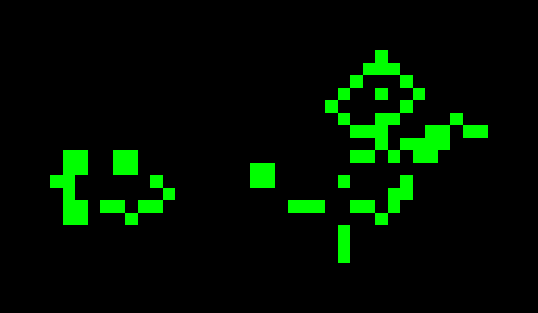
\includegraphics[scale=0.25]{life1-cropped.png}
		\hspace{3mm}
		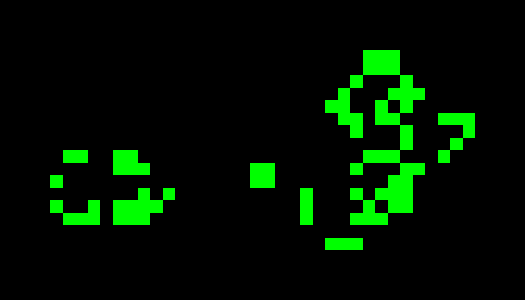
\includegraphics[scale=0.25]{life2-cropped.png}
	\begin{itemize}
		\item A cellular automaton
		\item Cells can be alive or dead.
		\item Dead cells come to life if bordered by 3 living cells.  Living cells
		continue living only if bordered by 2 or 3 living cells.
	\end{itemize}
\end{frame}

\begin{frame}
	\frametitle{Why is the Game of Life Interesting?}
	\begin{itemize}
		\item Rules were carefully chosen to allow complex, hard-to-predict
		patterns to emerge.
		\item Turing Complete: Life patterns can be used to simulate
		logical operations, memory, etc.
		\item Shows how complex structures can emerge from very simple
		rules
		\item 2010: Self-replicating pattern discovered (it destroys the
		original pattern though)
		\item Fun to implement and watch
		%\includegraphics[scale=0.1]{tm-cropped.png}
	\end{itemize}
\end{frame}

\begin{frame}
	\frametitle{Implementing the Game of Life}
	{\bf ``Brute Force'' Algorithm}
	\begin{itemize}
		\item Represent the Life grid, which is infinite, as a 2D array in
		memory of limited size.  2 copies of it are needed
		\item Set living cells to 1 and dead cells to 0.
		\item For each generation, iterate through all the cells and compute
		their fate. 
	\end{itemize}
	
	{\bf HashLife Algorithm}
	\begin{itemize}
		\item A dynamic programming approach that can hugely reduce the
		number of calculations needed
		\item This approach is more complicated and may be difficult to
		parallelize
		%\item May use more or less memory than brute force, depending on the
		%grid
		%\item Use a quadtree data structure to recursively divide the grid
		%\item Compute the fate of grid regions many generations in advance
		%and cache the result
	\end{itemize}
	This presentation focuses on the brute force algorithm.
\end{frame}

\begin{frame}
	\frametitle{Sample Serial Implementation (``Brute Force'' Algorithm)}
	\begin{lstlisting}
void compute_next_generation(const unsigned char** grid_in, unsigned char** grid_out, int width, int height) {
	for (int y = 1; y < height - 1; y++) {
		for (int x = 1; x < width - 1; x++) {
			unsigned char num_neighbors =
				grid_in[y+1][x-1] + grid_in[y+1][x] + grid_in[y+1][x+1] + grid_in[y][x-1] + grid_in[y][x+1] + grid_in[y-1][x-1] + grid_in[y-1][x] + grid_in[y-1][x+1];
			grid_out[y][x] =  ((num_neighbors == 3) || (cell(x, y) && num_neighbors == 2));
		}
	}
}
\end{lstlisting}

\end{frame}

\begin{frame}
	\frametitle{Parallelization of the Game of Life}
	\begin{itemize}
		\item Highly data parallel problem
		\item No iteration of the loop depends on any prior iteration
	\end{itemize}
	\begin{center}
	{\bf Shared memory}
	\end{center}
	\begin{itemize}
		\item In class we learned how we can easily parallelize a loop by
		placing an OpenMP directive.  This is done in the next slide.
	\end{itemize}
	\begin{center}
	{\bf GPU}
	\end{center}
	\begin{itemize}
		\item Data parallel problems like this can be effectively solved
		on a graphics processing unit with the help of a framework such as
		CUDA.
	\end{itemize}
\end{frame}

\begin{frame}[fragile]
	\frametitle{Sample OpenMP Implementation}
	\begin{lstlisting}
void compute_next_generation(const unsigned char** grid_in, unsigned char** grid_out, int width, int height) {
	#pragma omp parallel for
	for (int y = 1; y < height - 1; y++) {
		for (int x = 1; x < width - 1; x++) {
			unsigned char num_neighbors =
				grid_in[y+1][x-1] + grid_in[y+1][x] + grid_in[y+1][x+1] + grid_in[y][x-1] + grid_in[y][x+1] + grid_in[y-1][x-1] + grid_in[y-1][x] + grid_in[y-1][x+1];
			grid_out[y][x] =  ((num_neighbors == 3) || (cell(x, y) && num_neighbors == 2));
		}
	}
}
\end{lstlisting}








\end{frame}

\begin{frame}
\frametitle{CUDA (Compute Unified Device Architecture)}
	\begin{itemize}
		\item A framework developed by Nvidia for doing
		general-purpose computing on their GPUs.
		\item Components 
			%\begin{tabular}{|c|c|} \hline
			%Device & A supported Nvidia GPU \\ \hline
			%Compiler & {\tt nvcc} \\ \hline
			%Libraries & {\tt libCuda}, {\tt libcudart} \\ \hline
			%Linux kernel module & {\tt nvidia} \\ \hline
			%\end{tabular
			\begin{itemize}
			\item Device: A supported Nvidia GPU
			\item Language: A C-like language for writing kernels
			(code that runs on the device)
			\item Compiler: {\tt nvcc}
			\item Libraries: {\tt libCuda}, {\tt libcudart}
			\item Driver (Linux kernel module): {\tt nvidia}
			\end{itemize}
		\item Closed source and does not work on ATI/AMD GPUs. However we do
		have it available to use on the LittleFe.
		\item We must rethink how the code is to be written because the CUDA
		architecture is very different from what we are used to.
	\end{itemize}
\end{frame}

\begin{frame}
	\frametitle{Conway's Game of Life in CUDA}
	\begin{itemize}
		\item Grid data must be transferred to the GPU using the CUDA API.
		If needed back on CPU, it must explicitly be sent back.
		\item The CUDA architecture uses a large number of extremely
		lightweight threads.  We should assign each element of the grid to 1
		thread.  
		\item The {\tt compute\_next\_generation()} function will launch a
		CUDA kernel with appropriate numbers of thread blocks and threads
		per thread block.
	\end{itemize}
\end{frame}

\begin{frame}[fragile]
	\frametitle{Sample CUDA Implementation (kernel only)}
	\begin{lstlisting}
__global__ void kernel(const unsigned char** grid_in, unsigned char** grid_out, int width, int height) {
	int x = (blockIdx.x * blockDim.x) + threadIdx.x;
	int y = (blockIdx.y * blockDim.y) + threadIdx.y;
	if (x > 0 && x < width - 1 && y > 0 && y < height - 1) {
		unsigned char num_neighbors = grid_in[y+1][x-1] + grid_in[y+1][x] + grid_in[y+1][x+1] + grid_in[y][x-1] + grid_in[y][x+1] + grid_in[y-1][x-1] + grid_in[y-1][x] + grid_in[y-1][x+1];

		grid_out[y][x] =  ((num_neighbors == 3) || (cell(x, y) && num_neighbors == 2));
	}
}
\end{lstlisting}

\end{frame}

\begin{frame}[fragile]
	\frametitle{Sample CUDA Implementation (kernel launch)}
	\begin{lstlisting}
void compute_next_generation(const unsigned char** grid_in, unsigned char** grid_out, int width, int height)
{
	dim3 block(16, 16, 1);
	dim3 grid(width / block.x, height / block.y, 1);
	kernel<<< grid, block>>>(grid_in, grid_out, width, height);
}
\end{lstlisting}

\end{frame}

\begin{frame}
	\frametitle{My Implementation}
	\begin{itemize}
		\item 2 executables: {\tt openmp-life} and {\tt cuda-life}
		\item Renders grid using OpenGL ({\tt glDrawPixels()})
		\item In {\tt cuda-life}, OpenGL pixel buffer object is shared with
		CUDA kernel
		\item Some support for opening files containing Life patterns.
		\item OpenMP implementation optimized by moving {\tt pragma} up one
		function so that when multiple generations are advanced, only
		lightweight synchronization is needed among the threads.
		\item The above is not possible for CUDA, which requires new kernel
		launch each generation.
	\end{itemize}
\end{frame}

\begin{frame}
	LittleFe hardware:  Intel Atom Processor (2 cores), Nvidia GPU (2
	multiprocessors)
	\frametitle{Performance Comparison: Big Grid}
	\begin{table}[H]
	\caption{Running time for the Turing Machine (1760x1696 grid)}
	\begin{tabular}{c|c|c|c|c|}
	& \multicolumn{4}{c}{\bf Number of Generations} \\ \hline
				& 1 & 10 & 100 & 1000
				\\ \hline
	{\tt openmp-life} (1 thread) & 35 ms & 355 ms & 3557 ms & 35621 ms \\ \hline
	{\tt openmp-life} (2 threads) & 18 ms & 181 ms & 1807 ms & 18163 ms \\ \hline
	{\tt cuda-life}   & 10 ms & 100 ms & 996 ms  & 9963 ms    \\ \hline
	\end{tabular}
	\end{table}
	\begin{itemize}
	\item OpenMP implementation achieves 1.96x speedup with 2 threads compared to 1.
	\item CUDA implementation completes in 55\% of the time of 2-thread OpenMP
	implementation! 
	\end{itemize}
\end{frame}
\begin{frame}
	\frametitle{Performance Comparison: Small Grid}
	\begin{table}[H]
	\caption{Running time for a 50x50 grid}
	\begin{tabular}{c|c|c|c|c|}
	& \multicolumn{4}{c}{\bf Number of Generations} \\ \hline
				& 1 & 100 & 10000 & 1000000 \\ \hline
	{\tt openmp-life} (1 thread)& 0 ms & 3 ms & 295 ms & 29503 ms \\ \hline
	{\tt openmp-life} (2 threads)& 0 ms & 2 ms & 345 ms & 36831 ms \\ \hline
	{\tt cuda-life}   & 0 ms & 2 ms & 280 ms  &  28286 ms    \\ \hline
	\end{tabular}
	\end{table}

	2 threads was slower than 1! Too many synchronizations were required.

	CUDA was still faster, but not by much.  Launching a CUDA kernel requires
	some overhead.
\end{frame}

\begin{frame}
	\frametitle{Conclusion}
	{\bf Main Points}
	\begin{itemize}
		\item The LittleFe platform provided a way to test how Conway's Game of
		Life can be accelerated using OpenMP or CUDA.
		\item On large grids, both methods accelerate the computation
		compared to the sequential version, but CUDA did better.
		\item On very small grids, neither is much better than the serial,
		CPU version.  Most interesting patterns need large grids,
		though.
	\end{itemize}

	{\bf Further Research}
	\begin{itemize}
		\item Can the HashLife algorithm be parallelized?  With OpenMP? With CUDA?
		With MPI?
	\end{itemize}
\end{frame}

\begin{frame}
\frametitle{References}
\nocite{gol}
\nocite{tm}
\nocite{cuda_prog_guide}
\nocite{wolfram}
\bibliographystyle{plain}
\bibliography{refs}
\end{frame}

\end{document}
